% !TeX program = xelatex
\documentclass{assignment}
\usepackage[UTF8,scheme=chinese,fontset=none]{ctex}
\setCJKmainfont[Path=../assets/fonts/,BoldFont=FandolSong-Bold.otf,ItalicFont=FandolKai-Regular.otf]{FandolSong-Regular.otf}
\setCJKsansfont[Path=../assets/fonts/,BoldFont=FandolHei-Bold.otf]{FandolHei-Regular.otf}
\setCJKmonofont[Path=../assets/fonts/]{FandolHei-Regular.otf}
\usepackage{cite}
\graphicspath{{figures/}}
\geometry{a4paper}
\floatname{algorithm}{算法}
\crefname{figure}{图}{图}
\crefname{table}{表}{表}
\crefname{equation}{式}{式}
\crefname{section}{节}{节}
\renewcommand{\figurename}{图}
\renewcommand{\tablename}{表}
\renewcommand{\contentsname}{目录}
\renewcommand{\refname}{参考文献}
\setlength{\parindent}{2em}
\setlength{\parskip}{0.3em}
\makeatletter
\setlength{\@fptop}{0pt}
\setlength{\@fpsep}{12pt}
\setlength{\@fpbot}{0pt plus 1fil}
\makeatother
\renewcommand{\topfraction}{0.95}
\renewcommand{\bottomfraction}{0.95}
\renewcommand{\textfraction}{0.04}
\setlength{\textfloatsep}{12pt plus 2pt minus 2pt}

\hypersetup{pdftitle={基于TabPFN与ExtraTrees融合的药物溶解度预测},pdfauthor={COMP6133课程项目}}

\title{药物溶解度预测\\基于TabPFN与ExtraTrees的异质融合}
\author{COMP6133 机器学习课程项目}
\date{2026年11月18日}
\begin{document}
\maketitle
\tableofcontents
\newpage
\section*{摘要}
药物母体采样不均与条件测量重复，使溶解度模型需要同时处理结构差异和温度响应的跨药物迁移。本文提出SOLAR（溶曜）母体均衡结构--温度分解框架：SOLAR-H以树集成学习结构基线，通过组合内回归估计温度响应，并由分组验证选择响应增益；SOLAR-N以双分子编码器和温度差分监督实现联合学习。基于1904条记录，在1507条开发记录、128个母体上开展嵌套分组验证，比较12种方法。SOLAR-H的母体等权MAE为0.7164，相对ExtraTrees的配对误差差为-0.0305，95\%区间为[-0.0693, 0.0086]。固定配置消融中，将温度增益设为1使MAE增加0.0987，支持通过收缩控制条件响应的迁移误差。特征归因与组合固定效应分析表明，结构信息主导当前预测，而组合内温度关联与跨药物预测收益具有不同含义。该框架为小样本条件溶解度建模提供了兼顾母体均衡与响应调节的实现方式。

\noindent\textbf{关键词：}药物溶解度；母体均衡；结构交互；温度收缩；分组验证

\section{引言}
药物在不同溶剂中的溶解度影响溶剂筛选、结晶分离与制剂开发。实验难以覆盖全部药物、溶剂和温度组合，因此结构驱动的预测可为候选条件筛选提供参考\cite{bigsoldb2025,fastsolv2025}。实际数据中，同一药物常在多个条件下重复出现，逐行样本量也不能等同于独立分子的覆盖范围。

本文关注的任务是预测未见药物母体的条件溶解度。按记录随机划分可能让同一母体同时进入训练和验证，夸大对新药物的推广能力\cite{leakage2023}。另一方面，手工描述符、分子交互与温度信息之间存在非线性关系，仅增加模型结构复杂度未必能改善有限母体上的泛化。

TabPFN通过表格基础模型为小数据回归提供了不同于常规从零训练的方法\cite{tabpfn2025}；ExtraTrees以随机化树集成建模数值特征间的非线性关系\cite{extratrees2006}。两种模型的学习方式不同，因而值得在一致的分组协议下检验其互补性。本文以TabPFN＋ExtraTrees凸组合为主方法，通过内层母体验证同时组织基模型选择与融合选权。方法采用已有模型的任务化组合，不将异质融合本身宣称为原创算法。

本文首先分析数据覆盖与采样不均，随后给出双分支表示、母体加权树训练和折外选权流程，并与SOLAR结构--温度分解、通用回归器及多分支组合比较。模型比较同时考察母体与逐行误差，以检验融合收益及其在不同药物间的稳定性。

\section{相关工作}
\subsection{分子表示与条件溶解度建模}
分子描述符通过分子量、脂溶性、极性表面积和氢键能力等固定统计量表征结构；扩展连接指纹则通过局部原子邻域编码分子连接模式\cite{ecfp2010}。分子预训练进一步从大量无标签结构学习表示，例如MolCLR利用对比学习改善分子表征\cite{molclr2022}。对于多溶剂预测，单独表达溶质并不充分，MolMerger通过显式溶质--溶剂相互作用构造图表示\cite{molmerger2024}，说明两个分子之间的关系本身具有建模价值。

温度条件提供了另一类信息。FASTSOLV将分子表示、溶剂和温度联合建模，并利用温度梯度监督改善响应学习\cite{fastsolv2025}。本文据此以相邻温度观测差分补充逐点监督，并将其与母体均衡、结构交互和显式温度响应结合。

溶解度数据研究同时强调测量条件、离子状态和数据重叠对模型评价的影响\cite{solubility2024,bigsoldb2025}。这使分组划分和条件信息处理成为模型比较的重要组成部分。

近年来，分子表示学习进一步向几何信息和多模态知识扩展。Wang等总结了自监督学习与几何深度学习在科学发现中的作用，强调结构信息与数据表示之间的联系\cite{discovery2023}。MoleculeSTM通过对比学习对齐分子结构和文本描述，支持基于文本的分子检索与编辑\cite{moleculestm2023}，为结构分支引入化学语义提供了进一步方向。

\subsection{小样本表格学习与分组评价}
岭回归通过二次正则化控制参数方差\cite{ridge1970}；随机森林和ExtraTrees利用树集成拟合非线性关系\cite{randomforest2001,extratrees2006}；梯度提升通过逐步拟合残差优化目标函数\cite{boosting2001}。这些方法对中低维描述符具有直接适用性，也构成检验新模型的必要基线。

深度表格学习的近期进展表明，训练配置和评价协议会影响树模型与神经网络之间的比较\cite{tabular2021,trees2022}。RealMLP结合数值预处理、参数化和优化策略构建竞争力较强的MLP\cite{realmlp2024}；TabM通过参数高效集成产生多个成员预测\cite{tabm2025}。TabPFN进一步展示了表格基础模型在小数据任务上的潜力\cite{tabpfn2025}。本文选用TabM与RealMLP作为近期基线，并设置同规模MLP对照，以比较架构、条件监督和母体均衡的作用。

当同一对象在多个条件下重复出现时，随机划分记录可能使训练与验证共享对象信息。科学机器学习中的数据泄漏研究指出，评价单位应与实际推广任务匹配\cite{leakage2023}。因此，本文将药物母体作为划分单位，使用母体等权误差作为主要评价指标，并将训练损失中的均衡原则与之对应。

\subsection{模型解释与因果敏感性}
SHAP将预测分解为特征贡献，TreeSHAP使该思想能够高效应用于树模型\cite{shap2017,treeshap2020}；积分梯度则沿基准输入到观测输入的路径积分梯度，为神经网络提供输入归因\cite{integratedgradients2017}。本文分别解释混合模型的结构树分支与交互网络，并以整组置换比较完整预测函数对药物、溶剂和温度的依赖。

预测归因回答模型如何利用输入，因果分析还涉及干预定义与混杂控制\cite{causal2021}。本文以组合固定效应研究温度关联，再使用偏$R^2$参数化的遗漏变量偏差分析\cite{sensitivity2020}，定量说明未观测因素需要多强的关联才能改变该系数。

\section{数据预处理与探索性分析}
\subsection{数据结构与处理原则}
数据集包含1904条记录和7个字段，分别为药物名称、溶剂名称、药物SMILES、溶剂SMILES、温度、溶解度对数及溶解度单位。目标记为$y=\mathrm{Solubility\_log10}$，浓度显示采用$10^y$，其单位按数据表中的mol/L解释。温度按数据集数值尺度建模和绘图，原表未标注单位。

全量结构检查得到168种药物结构、49种溶剂结构及646种精确药物--溶剂组合。全部SMILES可解析，模型输入字段未发现缺失值。药物名称共有186种，其中17种结构对应多个名称，因此以结构识别建模对象，名称用于展示。

质量检查发现4条多余的完全重复记录；86组相同结构与温度条件存在不同标签，涉及205条记录，其中11组标签范围超过1个log10单位。另有26种药物结构包含多个片段。

\subsection{异常记录识别与处理}
如图\ref{fig:v2outliers}所示，采用箱线图的$1.5\,\mathrm{IQR}$规则标记开发集极端值，识别界限为$[Q_1-1.5\,\mathrm{IQR},Q_3+1.5\,\mathrm{IQR}]$。溶解度的界限为$[-4.633,2.599]$，共有11条记录位于界限之外；温度界限为$[10,50]$，共标记228条记录。箱线图的界限描述数值分布，不能单凭该界限判定测量错误；本研究将界限外记录标记后纳入训练，以保留低溶解度端和少见温度条件的覆盖。

处理流程首先核验缺失值、数值有限性和SMILES可解析性，再标记重复、标签冲突及箱线图极端值。完全重复记录和同条件冲突标签均保留参与主模型拟合；神经模型采用Huber损失减弱大残差的影响，树模型采用母体均衡权重控制高频药物的总贡献。构造温度差分时，同一组合在相同温度下的标签取均值，原始逐点训练记录保持完整。
\begin{figure}[htbp]\centering
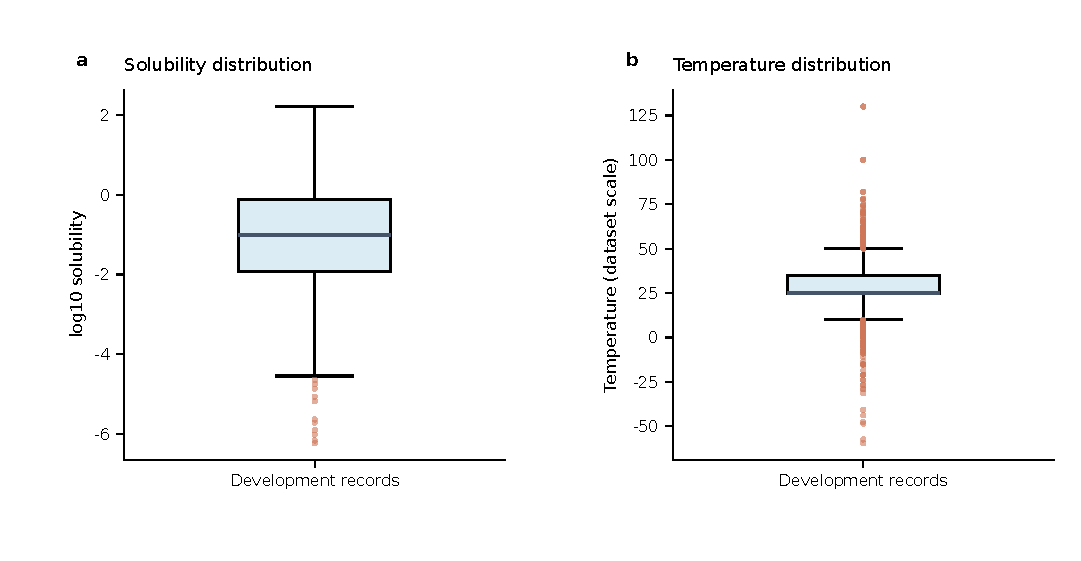
\includegraphics[width=\linewidth]{revision_v2/v2_outliers.pdf}
\caption{开发集极端值识别。箱体表示四分位区间，中线为中位数，须延伸至$1.5\,\mathrm{IQR}$范围内的最远观测，散点表示界限外记录。\textbf{a} 溶解度；\textbf{b} 温度。溶解度的界限外观测集中在低值端，温度的界限外观测分布于两端，反映两类变量不同的尾部结构。}\label{fig:v2outliers}
\end{figure}

\subsection{分子表示与药物母体分组}
每个分子提取11项描述符：分子量、MolLogP、拓扑极性表面积、氢键供体数、氢键受体数、可旋转键数、环数、芳香环数、重原子数、$sp^3$碳比例和形式电荷。药物与溶剂各提供11维，加入温度形成23维基础输入。对于需要标准化的模型，变换仅在训练折内拟合；本文提出模型采用
\begin{equation}
\tilde x_{ij}=\frac{x_{ij}-\mu_j^{(\mathrm{tr})}}{\sigma_j^{(\mathrm{tr})}},
\end{equation}
零方差维度的尺度取1。结构相似度分析另采用半径2、长度1024的Morgan指纹，以Tanimoto系数描述验证药物与训练结构的接近程度。

用于划分的母体键先通过RDKit的ChargeParent获得母体，再移除立体标记，共形成161组。该键将部分盐形式和立体变体归入同组，模型仍读取原始完整分子。数据划分包括1507条开发记录、128个母体，以及397条固定评价记录、33个母体。

\subsection{分布、覆盖与建模启示}
在168$\times$49种可能的结构组合中，仅646种有观测，覆盖率为7.85\%。222种重复组合包含1480条记录，占总数据的77.73\%。重复组合提供条件变化信息，而稀疏的组合覆盖使跨药物推广依赖于结构关系的学习。

温度范围为$-59.5$至130，中位数为25；目标范围为$-6.2343$至$2.2168$。图\ref{fig:v2data}展示结构覆盖、开发目标分布、条件分布和母体记录量。记录集中在少数母体与常见温度，逐行误差因而容易受到高频药物影响。本文将母体等权风险用于训练和评价，使低频药物同样影响总体目标。

\begin{figure}[htbp]\centering
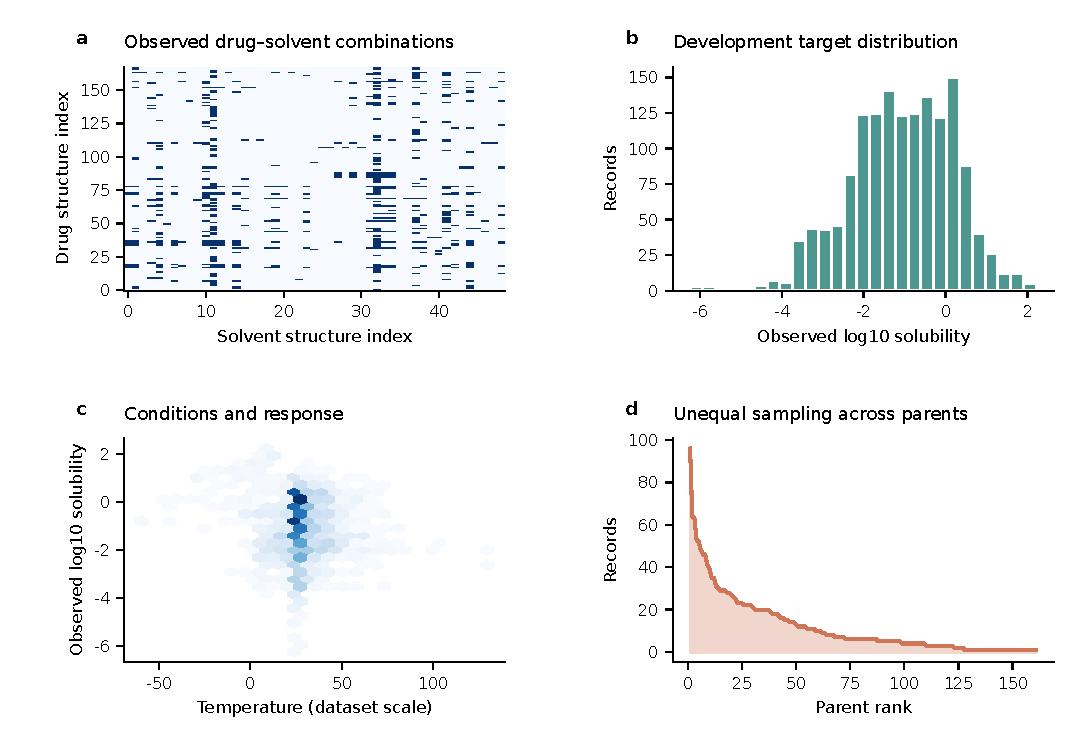
\includegraphics[width=\linewidth]{revision_v2/v2_data.pdf}
\caption{数据结构与探索性分析。\textbf{a} 全部1904条记录的结构组合覆盖，每个单元表示某药物与溶剂组合是否出现。\textbf{b,c} 1507条开发记录的目标分布及温度--目标分布，六边形颜色表示观测密度。\textbf{d} 161个母体按记录数降序排列的采样分布。组合覆盖稀疏且母体记录量差异明显，说明逐行样本量不能替代独立药物覆盖，支持采用母体均衡评价。}
\label{fig:v2data}\end{figure}

同一组合的温度序列则提供了结构间比较无法替代的信息。开发集中，157种组合具有温度变化，对应1118条记录和73个母体。对于同一组合，分子描述符保持不变，两次观测之差主要表达条件变化与实验差异。这些序列为从结构差异中分离温度响应提供了训练信息。


描述符关联进一步揭示了结构与条件信息的不同作用。开发记录中，药物氢键受体数、极性表面积和分子量与目标的Spearman相关系数分别为$-0.496$、$-0.465$和$-0.452$，温度的整体系数为$-0.025$。图\ref{fig:v2associations}给出描述符间关系及药物描述符与目标的关联。结构描述符与目标的关联强于总体温度关联，因而需要进一步在组合内部考察条件响应。

\begin{figure}[htbp]\centering
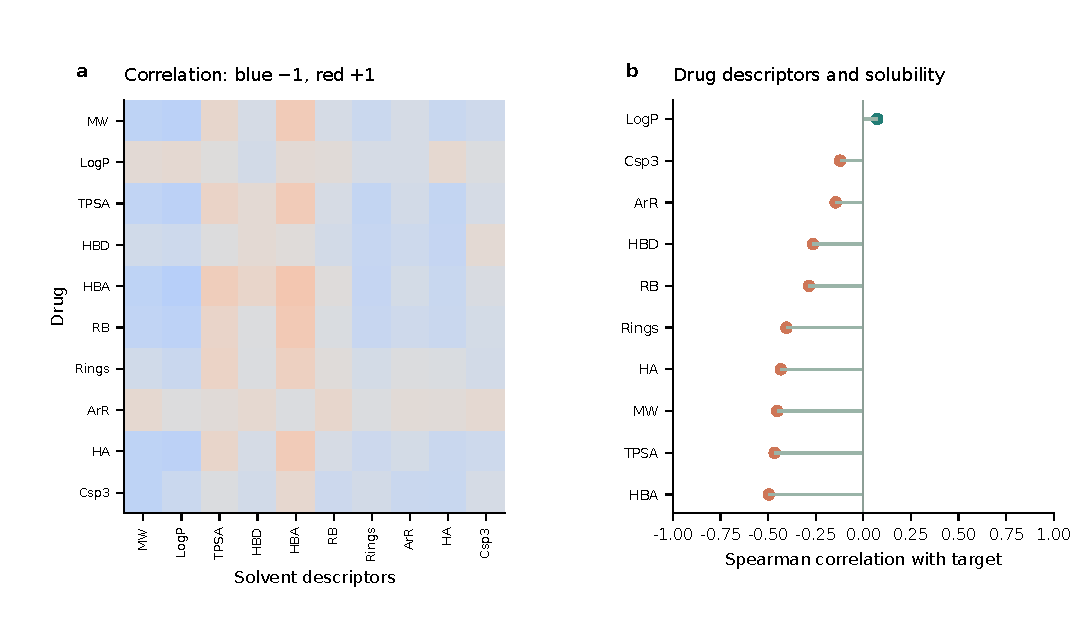
\includegraphics[width=\linewidth]{revision_v2/v2_associations.pdf}
\caption{开发集描述符关联。\textbf{a} 药物与溶剂描述符的Spearman相关矩阵，蓝色对应负相关，红色对应正相关，色阶固定为$[-1,1]$。\textbf{b} 药物描述符与溶解度的相关系数。MW为分子量，RB为可旋转键数，Rings为环数，ArR为芳香环数，HA为重原子数，Csp3为$sp^3$碳比例。药物极性及氢键相关描述符与目标的关联较强，提示结构基线是当前预测任务的重要信息来源。}
\label{fig:v2associations}\end{figure}

如图\ref{fig:v2samplingflow}所示，桑基图按照每个母体的记录数将数据分为1--5条、6--20条和超过20条三层，再连接到开发集与固定评价集。超过20条记录的高频层仅含30个母体，却贡献1078条记录；1--5条记录的低频层包含74个母体，仅贡献182条记录。两层在记录数与母体数上的反差，说明逐行训练会压低大量低频药物的相对贡献。
\begin{figure}[htbp]\centering
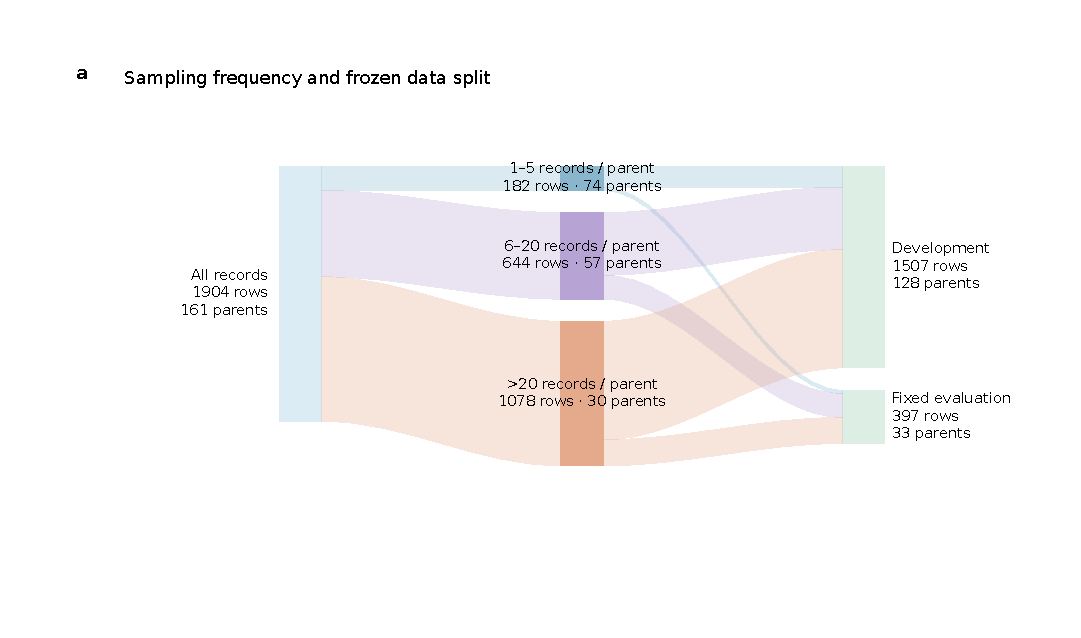
\includegraphics[width=\linewidth]{revision_v2/v2_sampling_flow.pdf}
\caption{采样频次与数据划分桑基图。中间节点依据全量数据的母体记录数分层；流带宽度与记录数成正比，节点标注记录数与独立母体数。高频层的30个母体贡献1078条记录，直观显示记录数量集中于少数药物母体。}\label{fig:v2samplingflow}
\end{figure}

上述分析确定了三个建模环节：按母体均衡训练贡献，以药物--溶剂交互表达组合关系，并从组合内变化学习温度响应。下一章将这些环节写入统一预测分解，再通过增益选择控制温度信息的迁移强度。

\section{TabPFN 与 ExtraTrees 融合方法}
\subsection{条件回归与原始模型}
记第 $i$ 条记录的药物和溶剂结构为 $d_i$ 与 $s_i$，温度为 $T_i$，母体分组为 $g_i$。模型使用两种结构和 CSV 原始温度预测对数溶解度 $y_i$。同一药物--溶剂组合在多个温度下有观测时，两种分子结构保持固定。原始模型 SOLAR-H 利用这一点，将预测写为
\begin{equation}
\hat y_{{\rm H},i}=b(z_i)+\gamma\,\tau_i\,\beta^\top u_i,\qquad u_i=[1;z_i],
\end{equation}
其中 $z_i$ 为结构特征，$\tau_i$ 为按训练折标准化的温度，$b$ 为 ExtraTrees 结构基线，$\gamma$ 为内层验证选择的温度增益。同一组合 $c$ 的 $z_i$ 固定，在组合内中心化可以消去 $b$。代码据此用有效温度偏差 $|\tau_i-\bar\tau_c|>10^{-9}$ 的记录拟合岭回归，得到 $\beta$：
\begin{equation}
\hat\beta=\arg\min_\beta
\sum_i w_i\big[(y_i-\bar y_{c(i)})-(\tau_i-\bar\tau_{c(i)})\,\beta^\top u_i\big]^2
+\lambda\|\beta\|_2^2 .
\end{equation}
求和仅覆盖上述有效记录，$\bar y_c$ 与 $\bar\tau_c$ 为该组合在训练折内的均值。给定 $\gamma$ 后，树在温度修正后的目标 $y_i-\gamma\tau_i\hat\beta^\top u_i$ 上拟合结构基线。后续的融合方法将温度与分子描述符一并输入两个学习器，由树切分和表格上下文建模条件关系。

\subsection{分子描述符与交互特征}
令 $\phi_k(m)$ 为分子 $m$ 的 $k$ 项描述符。每条记录的基础特征为 $[\phi_{11}(d_i);\phi_{11}(s_i);T_i]$，共 $2\times11+1=23$ 维。额外纳入完整 RDKit 描述符时，令 $D_i=\phi_{217}(d_i)$、$S_i=\phi_{217}(s_i)$，则基础拼接扩展至 $2\times217+1=435$ 维。为显式表示同类描述符的共同变化及差异，在此基础上拼接逐元素乘积与绝对差：
\begin{equation}
x_i^{\rm int}
=[D_i;S_i;T_i;D_i\odot S_i;|D_i-S_i|]
\in\mathbb R^{869}.
\end{equation}
例如，药物和溶剂各自的 MolLogP 除原始值外，还生成乘积和绝对差两列。两种交互各增加 217 维。再加入标准化药物母体结构的 217 项描述符，得到 1086 维的候选表示。树分支对当前训练折拟合缺失描述符的中位数插补和零方差筛选，并将同一变换应用于验证折。

\subsection{按母体加权的 ExtraTrees 候选}
单纯按记录计数时，训练折中含 $n_g$ 条记录的母体会贡献 $n_g$ 次损失。对训练折 $\mathcal T$，记 $n_g(\mathcal T)$ 为母体 $g$ 的记录数，$N_{\mathcal T}$ 和 $G_{\mathcal T}$ 分别为总记录数和母体数。将样本权重设为
\begin{equation}
w_i(q)=\frac{n_{g_i}(\mathcal T)^{-q}}
{N_{\mathcal T}^{-1}\sum_{j\in\mathcal T}n_{g_j}(\mathcal T)^{-q}},
\qquad q\in\{0,1\}.
\end{equation}
当 $q=0$ 时每条记录权重为 1。当 $q=1$ 时，分母为 $G_{\mathcal T}/N_{\mathcal T}$，同一母体的权重之和为 $N_{\mathcal T}/G_{\mathcal T}$。在完整开发集上，每个母体的总权重为 $1507/128\approx 11.77$。

对树节点中的记录集合 $L$，加权平方损失为 $J_L(v)=\sum_{i\in L}w_i(y_i-v)^2$。令 $J_L'(v)=0$，得到叶预测 $\hat v_L=\sum_{i\in L}w_i y_i/\sum_{i\in L}w_i$。对候选切分 $L=L_{\rm left}\cup L_{\rm right}$，比较母节点与两子节点各自最小平方损失的差，选择降幅最大的候选切分。最终输出 300 棵树的叶预测均值。每棵树不限制深度，叶节点至少含 2 条记录，每次切分考虑 0.7 比例的特征。完整、交互及含母体描述符三种表示与两个 $q$ 值组合成六项候选，内层按母体等权绝对误差选择。该指标与树拟合时的平方损失分别用于模型选择和节点拟合。

\subsection{TabPFN 的上下文预测}
TabPFN 分支使用公开 v2 回归权重 $\theta$。对一个验证样本 $x$，其上下文 $\mathcal C_{\mathcal T}=\{(x_j,y_j):j\in\mathcal T\}$ 由当前训练折的描述符、温度及对数溶解度构成。点预测取条件预测分布的均值\cite{tabpfn2025}：
\begin{equation}
f_{\rm PFN}(x)=\mathbb E_{\theta}[Y\mid x,\mathcal C_{\mathcal T}].
\end{equation}
模型权重固定，上下文的训练记录等权输入。内层比较 23 维与 435 维表示，并为每种表示比较 2 或 4 个内部集成成员。

\subsection{内层折外选参和融合}
对每个外层训练集，按母体重新划分三折。每个分支的每项候选均对三折中的验证记录生成折外预测。合并三折后，分别以母体等权 MAE（式\ref{eq:parentmae}）选择两分支配置。记内层记录 $i$ 对应的所选分支预测为 $p_i$ 和 $t_i$。试用 TabPFN 权重 $a$ 时，该记录的误差为
\begin{equation}
y_i-\big[a p_i+(1-a)t_i\big]=(y_i-t_i)-a(p_i-t_i).
\end{equation}
因此，融合是否减少一条记录的绝对误差，取决于分支预测差 $p_i-t_i$ 对树分支残差 $y_i-t_i$ 的修正。以 $I_g$ 表示内层折外记录中属于母体 $g$ 的行，按母体汇总该绝对误差，得到选权问题
\begin{equation}\label{eq:selectblend}
\hat a=\arg\min_{a\in\{0,\,0.25,\,0.5,\,0.75,\,1\}}
\frac{1}{G_{\rm in}}\sum_{g=1}^{G_{\rm in}}
\frac{1}{|I_g|}\sum_{i\in I_g}|(y_i-t_i)-a(p_i-t_i)|.
\end{equation}
离散网格仅需比较五项候选，两个端点对应单分支。选定配置和权重后，以整个外层训练集分别拟合两分支，在外层验证母体上输出
\begin{equation}\label{eq:newblend}
\hat y(x)=\hat a f_{\rm PFN}(x)+(1-\hat a)f_{\rm ET}(x).
\end{equation}
每折由种子 2026 选定配置和权重，再以种子 2026、17、42 分别拟合并评分。部署时在完整开发集上重复三折选参和选权，得到 23 维、2 成员的 TabPFN 与 869 维、$q=1$ 的 ExtraTrees，权重分别为 0.25 和 0.75。

\section{实验设置}
\subsection{评价协议与模型选择}
主要评价在1507条开发记录、128个母体上进行。外层沿用固定的五折母体划分，每折均将验证母体整体排除在训练之外；内层采用三折分组验证选择参数，随机种子为2026。每个可调方法预设12个候选配置，均值预测器只有一个配置。每个外层折在参数确定后以2026、17、42三个种子重新训练并评价。内层验证采用合并折外预测的母体等权MAE选模，不简单平均各折分数。

描述符标准化、温度中心化、目标归一化、母体权重和温度对均仅从当前训练部分计算。397条固定评价记录用于检验不同划分下的预测表现，主要比较依据嵌套分组验证。部署配置通过完整开发集上的三折分组验证确定，并以种子2026训练。

\subsection{比较模型与参数预算}
比较包含均值预测、Ridge、随机森林、ExtraTrees、直方图梯度提升（HGB）、TabM、RealMLP、普通MLP、温度差分MLP及两条提出路线，其中混合路线包含固定增益对照SOLAR-H$_0$与自适应收缩模型SOLAR-H，共12种方法。SOLAR-H$_0$采用$\gamma=1$并独立搜索其余超参数；单因素温度增益对照另在SOLAR-H的固定配置下开展。全部使用相同23维基础描述符输入；提出方法在内部构造交互。普通MLP和温度差分MLP采用两个同宽隐藏层，后者仅增加差分监督，为网络路线提供直接控制。

TabM采用官方参数高效集成实现，固定120轮；RealMLP采用官方PyTabKit实现，固定128轮，并关闭内部验证及提前停止。SOLAR-N固定160轮。各方法获得相同数量的参数候选，但单次拟合计算量不同，因此同时报告训练与推理耗时。

各模型的参数范围如表\ref{tab:searchspace}所示。
\begin{table}[htbp]\centering\small
\caption{参数搜索范围。除均值预测外，每类方法使用12个候选；较大的离散空间按固定种子抽样，SOLAR-H遍历12种组合；参数仅由内层验证选择。}\label{tab:searchspace}
\begin{tabularx}{\linewidth}{lX}\toprule
模型 & 参数范围\\\midrule
Ridge & $\alpha$为$10^{-3}$至$10^4$的12个对数等距值\\
随机森林、ExtraTrees & 200棵树；深度$\{8,16,\mathrm{None}\}$；叶节点$\{1,2,4,8\}$；特征比例$\{0.7,1.0\}$\\
HGB & 200轮；叶节点$\{7,15,31\}$；学习率$\{0.03,0.07\}$；正则化$\{0.1,1,10\}$\\
TabM & 宽度$\{64,128\}$；dropout $\{0,0.1,0.2\}$；学习率$\{0.001,0.003\}$；16个成员\\
RealMLP & 宽度$\{64,96,128,192\}$；隐藏层数$\{1,2,3\}$\\
普通MLP & 宽度$\{32,64,128\}$；学习率$\{0.001,0.003\}$；权重衰减$\{0.001,0.01\}$\\
温度差分MLP、SOLAR-N & 宽度$\{32,64\}$；学习率$\{0.001,0.003\}$；差分权重$\{0.1,1,3\}$\\
SOLAR-H$_0$ & 200棵树；深度$\{8,16,\mathrm{None}\}$；叶节点$\{1,2\}$；斜率惩罚$\{1,10,100,1000\}$\\SOLAR-H & 温度增益$\{0,0.1,0.3,1\}$；深度$\{8,16,\mathrm{None}\}$；200棵树、叶节点1、斜率惩罚1000\\\bottomrule
\end{tabularx}\end{table}

\subsection{指标、消融与不确定性}
记评价集包含$N$条记录、$G$个药物母体，$y_i$与$\hat y_i$分别为观测值和预测值，$n_g$为母体$g$的记录数，$\bar y=N^{-1}\sum_i y_i$。所有误差基于溶解度的log10尺度计算。

母体等权平均绝对误差为
\begin{equation}
\mathrm{MAE}_{\mathrm{parent}}=\frac1G\sum_{g=1}^G\frac1{n_g}
\sum_{i:g_i=g}|y_i-\hat y_i|.
\end{equation}
该指标给予每个母体相同权重，衡量模型在不同药物间的平均预测表现，数值越小越好。

逐行平均绝对误差为
\begin{equation}
\mathrm{MAE}=\frac1N\sum_{i=1}^{N}|y_i-\hat y_i|.
\end{equation}
MAE表示每条观测的平均偏差，数值越小越好；记录较多的母体在这一指标中贡献更大。

均方根误差为
\begin{equation}
\mathrm{RMSE}=\sqrt{\frac1N\sum_{i=1}^{N}(y_i-\hat y_i)^2}.
\end{equation}
平方项提高了大残差的权重，因此RMSE用于考察极端预测误差，数值越小越好。

决定系数为
\begin{equation}
R^2=1-\frac{\sum_{i=1}^{N}(y_i-\hat y_i)^2}{\sum_{i=1}^{N}(y_i-\bar y)^2}.
\end{equation}
$R^2$衡量相对于观测均值预测的误差缩减，数值越大越好，理想值为1；负值表示平方误差超过均值参照。

计算效率采用平均拟合时间与每条记录的批量推理时间：
\begin{equation}
\bar t_{\mathrm{fit}}=\frac1K\sum_{k=1}^{K}t_{\mathrm{fit},k},\qquad
\bar t_{\mathrm{pred}}=\frac1K\sum_{k=1}^{K}\frac{1000t_{\mathrm{pred},k}}{N_k},
\end{equation}
其中$K=15$对应五折外层评价与三个种子，$t$以秒计，$N_k$为第$k$次验证的记录数，两个指标分别以秒和毫秒/条表示，数值越小表示相同设备下开销越低。

消融表中的误差变化定义为
\begin{equation}
\Delta\mathrm{MAE}_{\mathrm{parent}}=
\mathrm{MAE}_{\mathrm{parent}}^{\mathrm{variant}}-
\mathrm{MAE}_{\mathrm{parent}}^{\mathrm{reference}}.
\end{equation}
负值表示变体误差低于对应完整模型。每个种子先合并五折预测计算指标，再平均三个种子的指标；母体配对区间采用2000次母体bootstrap估计。

消融固定各外层折选出的配置，分别关闭母体均衡、交互项、温度分支及差分损失，另加入仅母体均衡的普通MLP。学习曲线在每个外层训练集中按母体抽取25\%、50\%和75\%的数据，验证部分保持不变。灵敏度实验分别改变差分权重、网络宽度与斜率正则化，其他参数沿用该折配置。

\subsection{训练环境}
训练环境如表\ref{tab:environment}所示。
\begin{table}[H]\centering
\caption{训练环境。}\label{tab:environment}
\begin{tabular}{ll}\toprule
项目 & 值\\\midrule
处理器 & Apple M4\\
内存 & 24 GiB\\
操作系统 & macOS 27.2.1（arm64）\\
计算设备 & CPU\\
数值线程数 & 2\\
Python & 3.12.12\\
环境管理 & uv\\
NumPy / pandas & 2.5.5 / 3.1.1\\
scikit-learn & 1.9.1\\
RDKit & 2026.9.2\\
PyTorch & 2.15.0\\
TabM / PyTabKit & 0.0.3 / 1.8.0\\
\bottomrule\end{tabular}\end{table}

\section{结果与分析}
\subsection{统一分组评价下的模型比较}
表\ref{tab:v2comparison}给出12种方法的完整比较。两条提出路线中，SOLAR-H的母体等权MAE较低，为0.7164；最强基线为ExtraTrees，对应0.7469。二者的母体配对误差差为-0.0305，95\% bootstrap区间为[-0.0693, 0.0086]，128个母体中有67个误差下降。误差差的区间跨零，且改善分布于约半数母体，表明平均收益伴随较大的药物间差异（图\ref{fig:v2comparison}）。

\begin{table}[htbp]\centering\small
\caption{主要嵌套评价与固定划分评价。主要指标先按种子计算再平均；固定划分列来自完整开发集训练后的397条固定记录。所有误差均使用log10尺度。}\label{tab:v2comparison}
\begin{tabular}{lrrrrr}\toprule
模型 & 母体MAE$\downarrow$ & MAE$\downarrow$ & RMSE$\downarrow$ & $R^2\uparrow$ & 固定母体MAE$\downarrow$\\\midrule
SOLAR-H & 0.716 & 0.752 & 1.002 & 0.388 & 0.759\\
ExtraTrees & 0.747 & 0.749 & 0.973 & 0.423 & 0.734\\
随机森林 & 0.759 & 0.770 & 0.993 & 0.400 & 0.791\\
TabM & 0.778 & 0.770 & 1.000 & 0.391 & 0.725\\
HGB & 0.789 & 0.744 & 0.953 & 0.446 & 0.810\\
RealMLP & 0.804 & 0.815 & 1.068 & 0.304 & 0.783\\
SOLAR-H$_0$ & 0.824 & 0.822 & 1.155 & 0.186 & 0.749\\
温度差分MLP & 0.837 & 0.795 & 1.051 & 0.327 & 0.844\\
普通MLP & 0.838 & 0.799 & 1.048 & 0.330 & 0.842\\
SOLAR-N & 0.888 & 0.848 & 1.284 & -0.012 & 0.756\\
Ridge & 0.895 & 0.956 & 1.235 & 0.070 & 0.985\\
均值预测 & 0.964 & 1.059 & 1.311 & -0.048 & 1.028\\
\bottomrule\end{tabular}\end{table}
表\ref{tab:v2comparison}中的排序差异反映了模型优化对象的不同。HGB取得较低的逐行MAE和RMSE，说明其迭代拟合残差的方式适合减少当前记录分布中的总体偏差；SOLAR-H在母体等权MAE上更优，则与其均衡训练目标一致。高频药物在逐行指标中具有较大影响，而SOLAR-H通过重加权提高低频母体的训练贡献，因此其主要价值体现在药物层面的平均表现。

Ridge仅表达描述符的加性线性关系，难以充分刻画结构性质与溶剂条件的非线性组合；随机森林、ExtraTrees和HGB的较低误差支持非线性分区的建模价值。SOLAR-H进一步将结构预测与温度响应分离，使结构树集成能够先学习主要的分子差异，再由验证风险决定条件分支的强度。固定配置消融中，关闭母体均衡使母体MAE升高，将温度增益设为1也明显增加误差，这两项对照分别检验均衡权重和响应收缩的作用，具体结果见表\ref{tab:v2ablation}。

TabM的参数共享集成和RealMLP的优化配置为描述符任务提供了较强的神经网络基线，但SOLAR-N未从双编码器与温度差分中获得相同收益。其误差分布出现较长右尾，最差母体MAE达到10.567，表明少数药物上的响应偏差对总体表现影响较大。由于SOLAR-N的预测含有$\tau r(z)$，结构斜率估计误差会随温度偏离参考值而放大；关闭温度分支后的改善与这一机制一致。SOLAR-H允许验证过程将温度增益降至零，从而提供了一条抑制此类误差传播的路径。

固定划分下，TabM的母体等权MAE最低，SOLAR-H的误差也高于ExtraTrees（表\ref{tab:v2comparison}）。排序随评价母体变化，说明模型对药物组成具有不同敏感性，也体现了多折分组评价对平均推广表现的检验价值。SOLAR-H平均拟合时间为0.698秒，ExtraTrees为0.106秒；增加响应估计和交互表示后，混合路线在当前规模下保持亚秒级拟合。
\begin{figure}[htbp]\centering
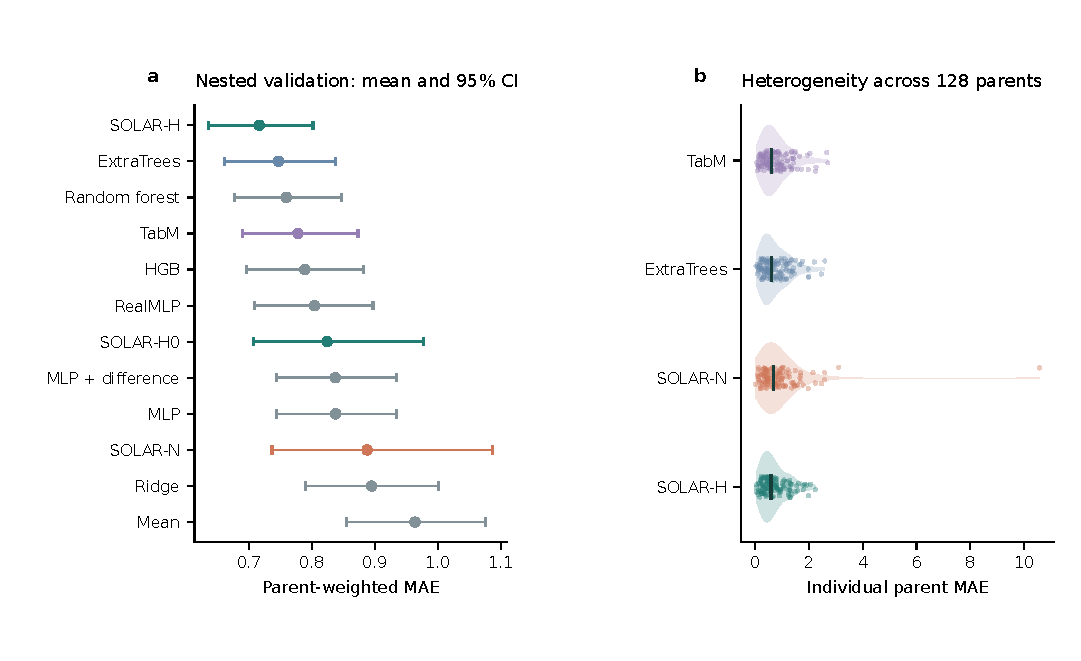
\includegraphics[width=\linewidth]{revision_v2/v2_comparison.pdf}
\caption{统一评价下的模型表现。\textbf{a} 128个母体的等权误差及2000次母体bootstrap的95\%区间。\textbf{b} 代表方法的母体误差分布，小点对应母体，短线表示中位数，密度形状描述分布。每个母体先平均三个种子的绝对误差。均值比较与母体分布共同呈现整体表现和误差集中程度。}
\label{fig:v2comparison}\end{figure}
\subsection{消融实验与数据规模}
如表\ref{tab:v2ablation}和图\ref{fig:v2ablation}所示，组件变体用于比较均衡权重、交互项及温度收缩的作用。
\begin{table}[htbp]\centering\small
\setlength{\tabcolsep}{5pt}
\caption{组件勾选消融结果。B为母体均衡，I为分子交互，T为温度分支，D为差分监督；$\checkmark$表示启用，--表示停用或不适用。$\gamma_{\rm CV}$表示沿用该外层折选定的增益，温度分支停用时增益记为0。误差差值以同路线完整模型为参照。}\label{tab:v2ablation}
\begin{tabular}{lcccccrr}\toprule
模型 & B & I & T & D & $\gamma$ & 母体MAE$\downarrow$ & $\Delta$MAE$\downarrow$\\\midrule
SOLAR-H$_0$ & $\checkmark$ & $\checkmark$ & $\checkmark$ & -- & $1$ & 0.8242 & +0.0000\\
SOLAR-H$_0$ & -- & $\checkmark$ & $\checkmark$ & -- & $1$ & 0.8407 & +0.0166\\
SOLAR-H$_0$ & $\checkmark$ & -- & $\checkmark$ & -- & $1$ & 0.7581 & -0.0660\\
SOLAR-H$_0$ & $\checkmark$ & $\checkmark$ & -- & -- & $0$ & 0.7131 & -0.1110\\
SOLAR-H & $\checkmark$ & $\checkmark$ & $\checkmark$ & -- & $\gamma_{\rm CV}$ & 0.7164 & +0.0000\\
SOLAR-H & -- & $\checkmark$ & $\checkmark$ & -- & $\gamma_{\rm CV}$ & 0.7380 & +0.0216\\
SOLAR-H & $\checkmark$ & -- & $\checkmark$ & -- & $\gamma_{\rm CV}$ & 0.7131 & -0.0033\\
SOLAR-H & $\checkmark$ & $\checkmark$ & -- & -- & $0$ & 0.7088 & -0.0076\\
SOLAR-H & $\checkmark$ & $\checkmark$ & $\checkmark$ & -- & $1$ & 0.8151 & +0.0987\\
SOLAR-N & $\checkmark$ & $\checkmark$ & $\checkmark$ & $\checkmark$ & $1$ & 0.8878 & +0.0000\\
SOLAR-N & -- & $\checkmark$ & $\checkmark$ & $\checkmark$ & $1$ & 0.8406 & -0.0472\\
SOLAR-N & $\checkmark$ & -- & $\checkmark$ & $\checkmark$ & $1$ & 0.8791 & -0.0087\\
SOLAR-N & $\checkmark$ & $\checkmark$ & -- & $\checkmark$ & $0$ & 0.8219 & -0.0659\\
SOLAR-N & $\checkmark$ & $\checkmark$ & $\checkmark$ & -- & $1$ & 0.8896 & +0.0017\\
\bottomrule\end{tabular}\end{table}

固定增益对照SOLAR-H$_0$关闭温度分支后，母体等权MAE由0.8242降至0.7131，提示结构相关斜率在未见母体上的迁移误差超过其带来的条件信息。SOLAR-H在五个外层折分别选择$\gamma=0,0,0.1,0.1,0$；完整开发集的选择为$\gamma=0$。在保持SOLAR-H其余参数不变时，将增益恢复为1使MAE增加0.0987，配对区间为[0.0221, 0.2327]。这一对照直接支持对温度分支进行收缩。

SOLAR-H移除母体均衡后，母体等权MAE增加0.0216；移除交互项或完全关闭温度分支则分别下降0.0033和0.0076。因此，当前结果支持均衡训练与保守使用温度信息，但未显示显式交互项的独立收益。SOLAR-N移除温度分支同样降低误差，而移除差分监督仅使MAE增加0.0017，表明差分监督对该网络平均误差的影响较小。

普通MLP加入母体均衡后，母体等权MAE由0.8379降至0.8261，低于SOLAR-N，说明均衡训练本身已有收益，增加交互编码与差分监督并未进一步降低误差。图\ref{fig:v2ablation}b中，两条学习曲线随训练母体增加而下降，且由75\%增至100\%时下降幅度收窄；SOLAR-H在四个比例下均保持较低误差。该结果体现混合路线在当前小样本范围内的样本效率，同时将进一步增加结构覆盖与扩大网络容量区分为两种不同的改进方向。
\begin{figure}[htbp]\centering
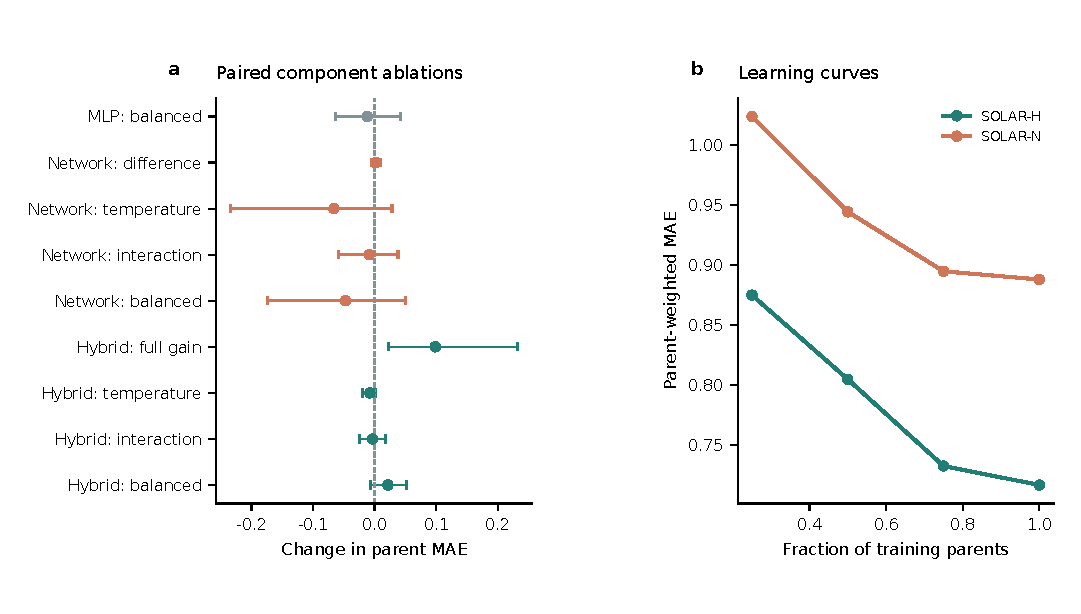
\includegraphics[width=\linewidth]{revision_v2/v2_ablation.pdf}
\caption{组件与数据规模分析。\textbf{a} 组件变体相对完整模型的配对母体误差差及95\% bootstrap区间；Full gain将温度增益恢复为1；MLP的均衡变体以普通MLP为参考。\textbf{b} 按母体抽取25\%、50\%、75\%及100\%训练数据的学习曲线，点为三个种子合并五折评价后的均值。两组实验分别考察组件取舍和独立药物覆盖对预测的影响。}
\label{fig:v2ablation}\end{figure}
\subsection{灵敏度与误差结构}
组件消融进一步引出参数强度的影响。图\ref{fig:v2sensitivity}中，SOLAR-N随差分权重变化的母体等权MAE为[0.8843, 0.8867]，SOLAR-H$_0$随斜率正则化变化的误差为[0.8162, 0.8494]；另行改变SOLAR-N宽度时，误差范围为[0.8455, 0.8964]。差分权重跨多个数量级时误差变化较小，而网络宽度的影响更大，说明当前网络的主要约束更可能来自表示容量与结构覆盖的匹配；固定增益模型即使加强斜率正则化，仍未达到SOLAR-H的母体误差水平，提示直接控制温度分支输出幅度具有额外作用。
\begin{figure}[htbp]\centering
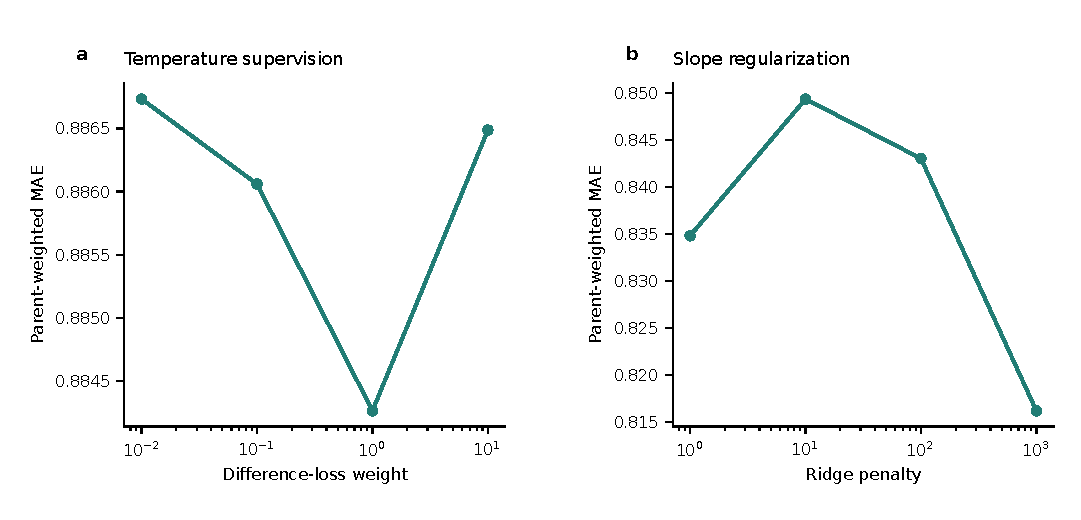
\includegraphics[width=\linewidth]{revision_v2/v2_sensitivity.pdf}
\caption{条件监督与斜率正则化的灵敏度。\textbf{a} 改变SOLAR-N的差分损失权重。\textbf{b} 改变SOLAR-H$_0$的岭回归惩罚。其余参数保持各外层折选定配置，纵轴为三个种子的平均母体等权MAE。差分权重曲线较平缓，斜率正则化曲线呈非单调变化。}
\label{fig:v2sensitivity}\end{figure}
在参数层面的比较之后，图\ref{fig:v2errors}定位了SOLAR-H的误差分布。观测--预测图中，低溶解度端的预测向中心收缩，对应稀疏尾部样本的分辨能力较弱；单条记录跨种子的平均绝对误差最高为3.675。母体误差累积分布则将这种局部大误差与多数药物的表现区分开来。最大训练结构相似度与逐行绝对误差的Spearman系数为-0.062，表明相似结构也可能出现不同幅度的误差；因此，相似度适合作为结构接近程度的描述，不能直接替代预测误差评价。
\begin{figure}[htbp]\centering
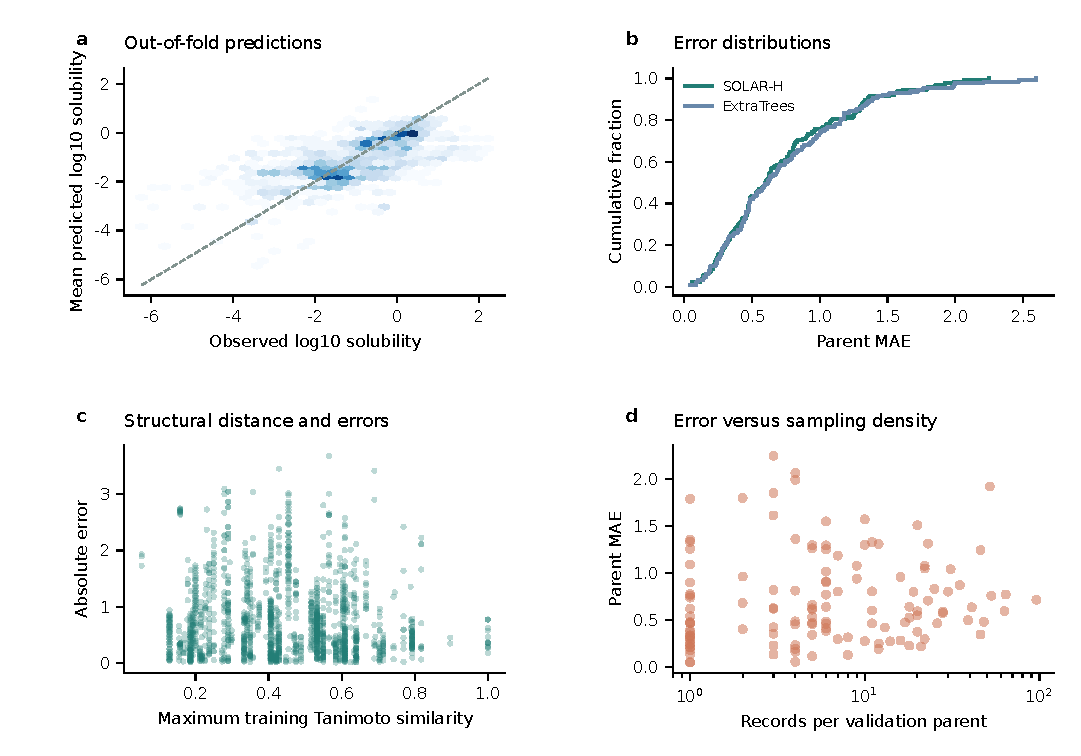
\includegraphics[width=\linewidth]{revision_v2/v2_errors.pdf}
\caption{主要提出方法的折外误差。\textbf{a} 观测与三个种子平均预测的hexbin图，虚线为一致线。\textbf{b} 母体误差的经验累积分布。\textbf{c} 最大训练结构相似度与逐行误差。\textbf{d} 验证母体记录量与母体误差。误差先在各训练种子计算绝对值后平均，区别于平均预测的绝对误差。低溶解度端偏离一致线，结构相似度与误差关系较弱。}
\label{fig:v2errors}\end{figure}
\subsection{结构与温度分支的可解释性}
误差分析描述预测偏差的位置，特征归因进一步考察模型依赖的信息。部署的SOLAR-H选择$\gamma=0$，其温度贡献及温度置换增量均为零。TreeSHAP作用于实际结构树分支，温度头贡献直接由$\gamma\tau r(z)$计算。结构分支平均绝对贡献最大的三个输入为\texttt{drug\_HBA}、\texttt{drug\_TPSA}、\texttt{drug\_RingCount}。SHAP贡献与期望值之和重构结构基线的最大绝对误差为$6.66\times10^{-15}$。

SOLAR-N采用1024段梯形数值积分计算积分梯度，参考输入为标准化描述符零向量和中心温度。完整网络的平均绝对归因最高的输入为\texttt{drug\_HBA}、\texttt{drug\_MolLogP}、\texttt{drug\_TPSA}；归因总和与相对基准预测差的最大误差为0.00522。图\ref{fig:v2explanations}c将单个预测展开为结构基准与各特征贡献，显示局部结果由多项结构信息共同形成；图\ref{fig:v2explanations}d的整组置换进一步显示，打乱药物描述符带来的误差增加大于打乱溶剂或温度。两种归因方法均将氢键受体数与极性相关描述符排在前列，说明模型主要利用分子极性和氢键能力区分溶解度；该解释与SOLAR-H将结构基线作为主要预测分量的设计一致。
\begin{figure}[htbp]\centering
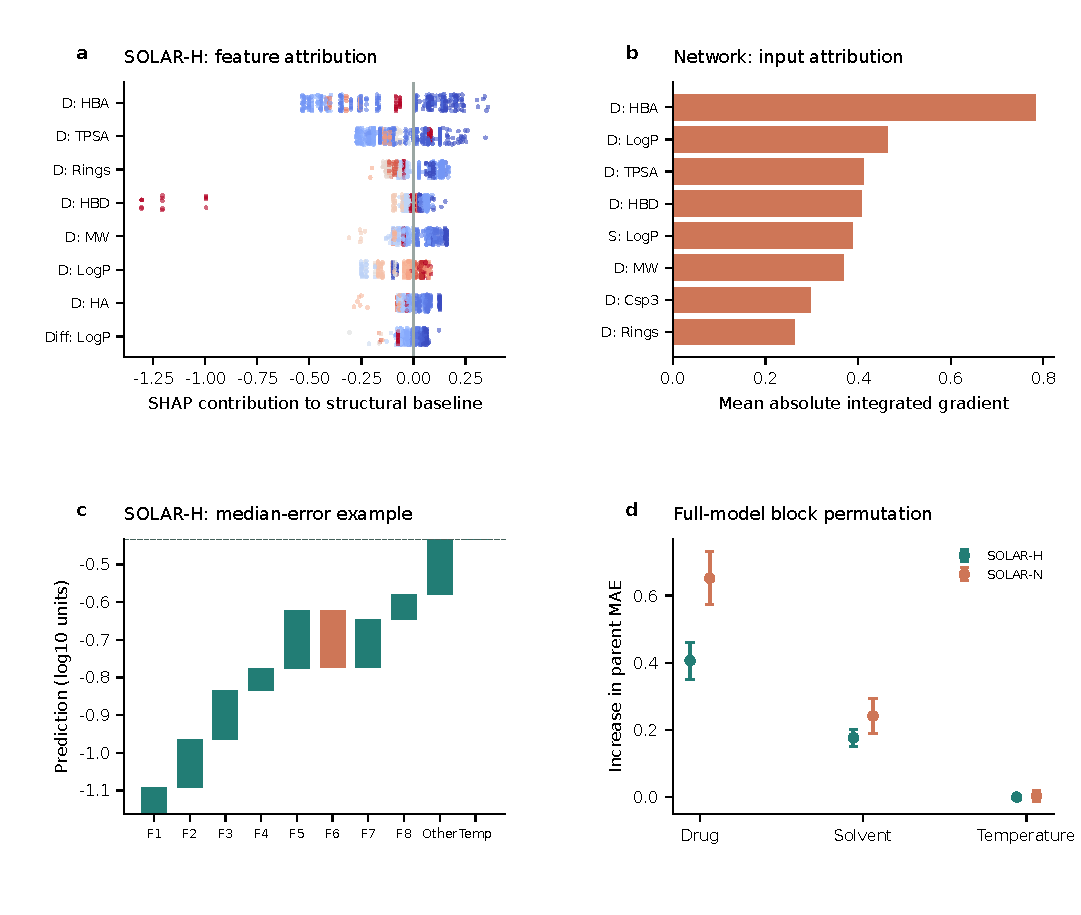
\includegraphics[width=\linewidth]{revision_v2/v2_explanations.pdf}
\caption{提出模型的可解释性。\textbf{a} 混合模型结构基线的前八项平均绝对SHAP特征，红色为高特征值、蓝色为低特征值；D、S、Prod、Diff分别表示药物、溶剂、乘积与绝对差。\textbf{b} SOLAR-N完整预测的积分梯度。\textbf{c} 固定评价集中混合模型绝对误差居中的样本，F1--F8对应a中顺序，Other汇总其余结构特征，Temp为温度头；起点为结构分支期望值。\textbf{d} 完整模型的特征组置换，点与误差线为20次置换的均值和标准差。解释样本为相同397条固定评价记录。全局排序、局部贡献与整组置换从不同尺度描述模型的信息依赖。}
\label{fig:v2explanations}\end{figure}
\subsection{温度关联与因果敏感性}
温度在预测中的贡献较小，还需结合组合内关联解释。图\ref{fig:v2causal}a给出分析假设：药物与溶剂结构影响测量温度的选择和溶解度，未测因素$U$同时影响二者。本文在开发数据上拟合组合固定效应模型$y_{ic}=\alpha_c+\beta T_{ic}+\epsilon_{ic}$，使用组合内去均值估计共同斜率。
157种具有温度变化的组合包含1118条记录、73个母体。在这些相同样本中，未调整组合的斜率为-0.00746，组合内斜率为0.01538；后者的母体bootstrap区间为[0.01236, 0.01902]。逐一移除母体后的斜率范围为[0.01424, 0.01599]，逐一剔除后仍保持正关联。
进一步用偏$R^2$表示潜在未测变量的强度。设$R_T^2$为$U$与温度在控制组合后的偏$R^2$，$R_Y^2$为$U$与结果在控制组合和温度后的偏$R^2$，则遗漏变量导致的点估计偏差大小为\cite{sensitivity2020}
\begin{equation}
|\mathrm{bias}|=\mathrm{SE}_{\mathrm{OLS}}(\hat\beta)
\sqrt{\mathrm{df}\frac{R_Y^2R_T^2}{1-R_T^2}}.
\end{equation}
当两种关联强度相同，偏$R^2$约为0.540即可将当前正斜率调整至零。该数值刻画点估计对假设混杂的敏感性。该分析估计控制组合后的温度关联；实验来源、pH和固态信息未被观测，其潜在混杂作用由图\ref{fig:v2causal}c中的敏感性曲面表征。图\ref{fig:v2causal}揭示总体温度关联与组合内关联方向不同，说明药物和溶剂组成会影响温度趋势的解释；图\ref{fig:v2causal}d中的组合温度序列刻画局部响应，而SOLAR-H的增益由未见母体上的验证误差决定。两者分别对应组合内拟合与跨药物迁移，因而正温度关联与较小预测增益可以同时出现。
\begin{figure}[htbp]\centering
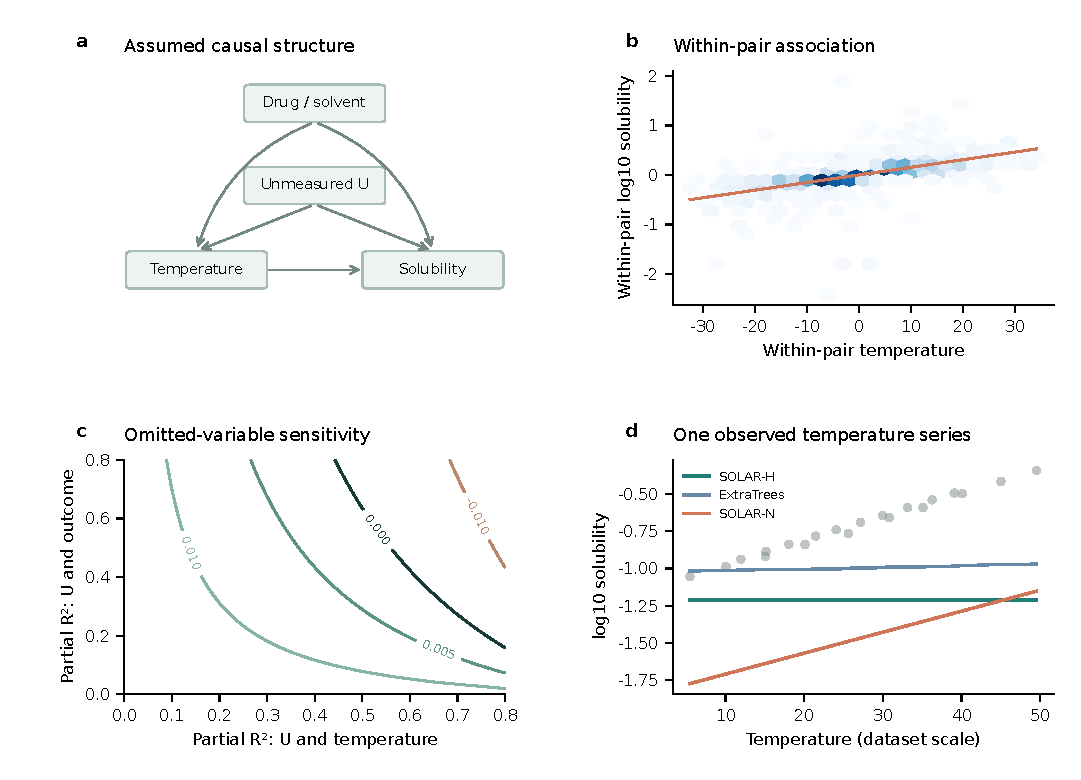
\includegraphics[width=\linewidth]{revision_v2/v2_causal.pdf}
\caption{温度关联、混杂敏感性与模型响应。\textbf{a} 分析采用的假设DAG。\textbf{b} 开发数据组合内去均值后的分布及共同斜率。\textbf{c} 未测变量不同偏$R^2$强度下向零方向调整的系数等高线，零线对应消除正关联所需的组合强度。\textbf{d} 温度覆盖较充分的一种开发组合的观测与模型响应。组合内斜率、混杂敏感性与单组合响应分别呈现温度分析的统计、假设和局部层面。}
\label{fig:v2causal}\end{figure}

\FloatBarrier
\section{模型评价与推广}
\subsection{模型优点}
\begin{enumerate}
\item SOLAR通过母体均衡权重协调不同采样频次药物对训练目标的贡献，使记录较少的药物也能参与模型优化，并与母体等权评价指标保持一致，为新药物条件下的溶解度估计提供统一的训练目标。
\item SOLAR-H将结构基线与温度响应分别建模，并通过内层分组验证选择温度增益，使条件信息的使用程度随数据证据调整，从而缓解固定温度分支带来的迁移误差，提升当前数据上的平均预测表现。
\item SOLAR-H使用低维分子描述符和树集成完成预测，在当前CPU环境下平均单次外层拟合约需零点七秒，能够以较低的计算成本完成多组参数比较，并支持交互应用中的连续条件探索与批量预测。
\item SOLAR的预测形式将结构贡献和温度贡献明确分开，可结合特征归因与响应曲线分析药物、溶剂及条件变化的作用，使预测结果便于追踪，也方便使用者在演示界面中比较不同模型的输出。
\end{enumerate}
\subsection{模型局限}
\begin{enumerate}
\item 当前数据中的独立药物母体和溶剂组合覆盖仍较有限，后续可增加不同化学类别及重复实验记录，使模型学习到更丰富的结构与条件关系，并通过新增来源的数据进一步考察预测表现的稳定性。
\item 目前输入主要由固定分子描述符与温度组成，后续可在数据条件允许时补充三维构象、酸碱条件和固态信息，以提高模型对具体实验体系的区分能力，并进一步丰富结构分支的表达方式。
\item 现有演示应用围绕数据集中已有的药物和溶剂提供选择与比较，后续可增加自定义分子输入、批量任务管理和结果检索等功能，使模型更便于融入不同规模的溶剂筛选与实验分析流程。
\end{enumerate}
\subsection{模型推广}
SOLAR-H适合用作候选药物与溶剂组合的初步排序工具，其母体均衡目标对应药物之间的平均预测质量。进一步推广可沿两条路径展开：利用来源明确的温度序列检验不同药物类别所需的收缩强度；将图表示或分子预训练嵌入结构分支\cite{molclr2022,molmerger2024}，在相同母体划分下比较其对低溶解度尾部误差的改善。前者检验条件响应的可迁移范围，后者检验更丰富表示能否补充当前描述符的信息。

\subsection{交互应用}
基于冻结模型构建的Solubility Studio采用英语为主、中文同步显示的界面，支持12种模型选择、药物与溶剂结构展示、单点预测、温度响应及多溶剂比较。两两对比使用完全相同的输入，展示预测差值、响应曲线、统一分组指标和母体误差散点；结果可导出为CSV。方法页面呈现两条算法路线和完整比较表。应用直接读取已训练模型及各自的预处理参数，将论文中的模型转化为可交互比较的预测工具。

\section{结论}
本文建立了从条件溶解度建模到交互预测的流程。按药物母体划分数据，并以母体等权 MAE 选择配置，使验证目标与未见母体预测任务一致。开发集比较中，TabPFN 与丰富描述符 ExtraTrees 的双分支组合取得最低观测误差。折间权重及低溶解度端误差表明，后续验证应关注融合收益在不同母体上的稳定性，以及低溶解度样本的预测校准。

\FloatBarrier
\newcommand{\BIBdecl}{\fontsize{10}{13}\selectfont\setlength{\itemsep}{0.1em}\setlength{\parsep}{0pt}}
\bibliographystyle{IEEEtran}
\bibliography{../bibliography/references}
\end{document}
